% !TeX root = ../main.tex

\subsection*{Isometric Feature Mapping (ISOMAP)}
A non-linearity ``patch'' to MDS

\begin{figure}[H]
	\centering
	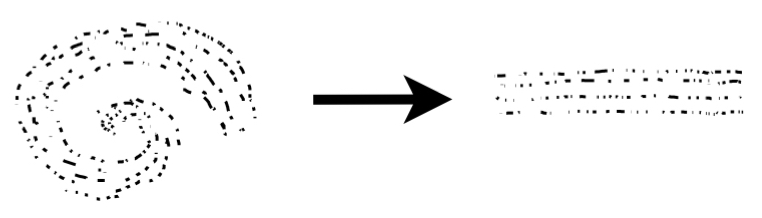
\includegraphics[width=0.5\textwidth]{isomap}
\end{figure}

\paragraph{Idea:} Nearby points have their ``usual'' euclidian distance. If a pair of points are not within a local neigbourhood, then the distance between these points is a \textbf{graph distance}\footnote{Compute the all pairs shortest path (Dejkstra, A*,  DFS, Floyd–Warshall, ...)}. Then run MDS on the resulting distance Matrix.

ISOMAP operates on geodesic distances (like a distance on earths surface/distances on the manifold).

\begin{itemize}
	\item ISOMAP is guaranteed asymptotically to recover the true dimensionality and geometric structure of a strictly larger class of nonlinear manifolds, which intrinsic geometry is that of a convex region of Euclidean space
	\item ISOMAP is a polynomial time, noniterative procedure which guarantees global optimality
\end{itemize}
